% hm-06-poststruct.tex

\documentclass[xcolor=dvipsnames]{beamer}

\usepackage{graphicx}
% \usepackage{wrapfig}
% \usepackage{colortbl}
\usepackage{alltt}
% \definecolor{myblue}{rgb}{0.8,0.85,1}

\mode<presentation>
{
  \usetheme{Warsaw}
  \setbeamercovered{transparent}
}
% \usecolortheme[named=OliveGreen]{structure}
\setbeamertemplate{navigation symbols}{} 
\setbeamertemplate{blocks}[rounded][shadow=true] 

\newif\ifBCITCourse
\BCITCoursetrue
\BCITCoursefalse
\newif\ifWhichCourse
\WhichCoursetrue
% \WhichCoursefalse
\ifBCITCourse
\ifWhichCourse
\newcommand{\CourseName}{Statistics for Food Technology}
\newcommand{\CourseNumber}{MATH 1441}
\newcommand{\CourseInst}{BCIT}
\else
\newcommand{\CourseName}{Calculus for Geomatics}
\newcommand{\CourseNumber}{MATH 1511}
\newcommand{\CourseInst}{BCIT}
\fi
\else
\newcommand{\CourseName}{Philosophy and Literature}
\newcommand{\CourseNumber}{PHIL 375}
\newcommand{\CourseInst}{UBC}
\fi

\title{Foucault and Co}
\subtitle{{\CourseNumber}, {\CourseInst}}

\author{\CourseName}

\date{November 2, 2017}

% \begin{frame}
%   \frametitle{iClicker Question One}
% Choose from the following options. This item will be graded.
% \begin{block}{iClicker Question}
  
% \end{block}
% \begin{description}
% \item[A\hspace{.2in}$\blacktriangleright$] 
% \item[B\hspace{.2in}$\blacktriangleright$] 
% \item[C\hspace{.2in}$\blacktriangleright$] 
% \item[D\hspace{.2in}$\blacktriangleright$] 
% \item[E\hspace{.2in}$\blacktriangleright$] 
% \item[F\hspace{.2in}$\blacktriangleright$] 
% \end{description}
% \end{frame}

% \begin{figure}[h]
% \includegraphics[scale=.3]{./extrema1.png}
% \end{figure}

\begin{document}

\begin{frame}
  \titlepage
\end{frame}

\begin{frame}
  \frametitle{Structuralism Table}
\begin{figure}[h]
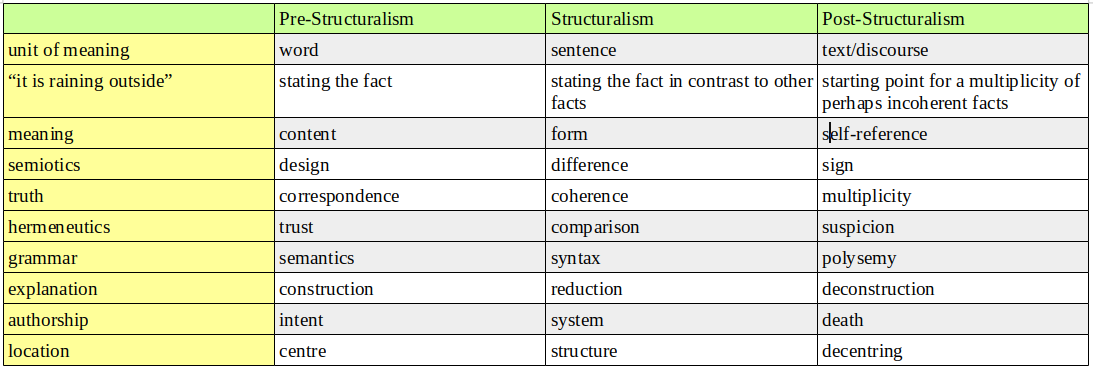
\includegraphics[scale=.3]{./structable.png}
\end{figure}
\end{frame}

\begin{frame}
  \frametitle{iClicker Question}
Choose from the following options. This item will be graded.
\begin{block}{iClicker Question}
What is the narrative eighty years after Damiens' execution to which
the public execution is set in contrast?
\end{block}
\begin{description}
\item[A\hspace{.2in}$\blacktriangleright$] the overcrowding of prisons
\item[B\hspace{.2in}$\blacktriangleright$] the abolition of the death penalty
\item[C\hspace{.2in}$\blacktriangleright$] a timetable of rules for young prisoners
\item[D\hspace{.2in}$\blacktriangleright$] institutional racism in prisons
\end{description}
\end{frame}

\begin{frame}
  \frametitle{iClicker Question}
Choose from the following options. This item will be graded.
\begin{block}{iClicker Question}
What does Foucault identify as a problem with modern discourse about sex?
\end{block}
\begin{description}
\item[A\hspace{.2in}$\blacktriangleright$] modernity is too
  body-focused (instead of mind-focused) in its sexuality
\item[B\hspace{.2in}$\blacktriangleright$] we talk about sexual desire too much
  (the endless mill of speech)
\item[C\hspace{.2in}$\blacktriangleright$] we don't talk about sex
  enough (repressed sexual desire must be articulated)
\item[D\hspace{.2in}$\blacktriangleright$] men want sex, women want
  conversation (gender imbalance with respect to verbal and sexual
  intimacy)
\end{description}
\end{frame}

\begin{frame}
  \frametitle{iClicker Question}
Choose from the following options. This item will be graded.
\begin{block}{iClicker Question}
According to Foucault, modern discourse about sex is intimately linked to
\end{block}
\begin{description}
\item[A\hspace{.2in}$\blacktriangleright$] the economic and political problem of population
\item[B\hspace{.2in}$\blacktriangleright$] the fear of sexually-transmitted disease
\item[C\hspace{.2in}$\blacktriangleright$] an erosion of monogamy due to homosexuality
\item[D\hspace{.2in}$\blacktriangleright$] the Christian dogma of the Trinity
\end{description}
\end{frame}

\begin{frame}
  \frametitle{iClicker Question}
Choose from the following options. This item will be graded.
\begin{block}{iClicker Question}
What, according to Foucault, is the relationship between knowledge and power?
\end{block}
\begin{description}
\item[A\hspace{.2in}$\blacktriangleright$] knowledge and power have separate domains
\item[B\hspace{.2in}$\blacktriangleright$] power corrupts knowledge
\item[C\hspace{.2in}$\blacktriangleright$] power produces knowledge, power and knowledge imply one another
\item[D\hspace{.2in}$\blacktriangleright$] knowledge constrains power
\end{description}
\end{frame}

% \begin{frame}
%   \frametitle{iClicker Question}
% Choose from the following options. This item will be graded.
% \begin{block}{iClicker Question}
%   Who is Herculine Barbin (Foucault uses her to show that categories
%   of sex are constructed through historically specific modes of
%   sexuality)?
% \end{block}
% \begin{description}
% \item[A\hspace{.2in}$\blacktriangleright$] a nineteenth-century hermaphrodite
% \item[B\hspace{.2in}$\blacktriangleright$] Foucault's mother
% \item[C\hspace{.2in}$\blacktriangleright$] a woman who was condemned
%   to death by hanging
% \item[D\hspace{.2in}$\blacktriangleright$] a French postmodern philosopher
% \end{description}
% \end{frame}

% \begin{frame}
%   \frametitle{iClicker Question}
% Choose from the following options. This item will be graded.
% \begin{block}{iClicker Question}
% Which three philosophers' views of sex does Butler describe in more detail?
% \end{block}
% \begin{description}
% \item[B\hspace{.2in}$\blacktriangleright$] Kant, Foucault, Derrida
% \item[C\hspace{.2in}$\blacktriangleright$] Kant, Hegel, Nietzsche
% \item[D\hspace{.2in}$\blacktriangleright$] Irigaray, Greer, Schwarzer
% \item[A\hspace{.2in}$\blacktriangleright$] Irigaray, Foucault, Wittig
% \end{description}
% \end{frame}

% \begin{figure}[h]
%   \includegraphics[scale=.3]{./belle.png}
% \end{figure}

% \begin{frame}
%   \frametitle{Footnotes}
% Having to read a footnote resembles having to go downstairs to answer the door while in the midst of making love. (Noel Coward)
% \end{frame}

\begin{frame}
  \frametitle{The Penal System: A Historical Disconitnuity}
  \begin{equation}
    \label{eq:zeiqueex}
    \begin{array}{rcl}
      \mbox{executioner} & \mbox{vs.} & \mbox{army of technicians} \\
      \mbox{punishment of body} & \mbox{vs.} & \mbox{suspension of rights} \\
      \mbox{individual (King and Condemned)} & \mbox{vs.} & \mbox{institution} \\
      \mbox{violence} & \mbox{vs.} & \mbox{bio-power} \\
      \mbox{theatre} & \mbox{vs.} & \mbox{order and silence (7)} \\
      \mbox{law and its subjects} & \mbox{vs.} & \mbox{norms and their subjects} \\
      \mbox{everyday perception} & \mbox{vs.} & \mbox{abstract consciousness (9)} \\
      \mbox{transcendental responsibility} & \mbox{vs.} & \mbox{responsibility relieved by} \\
      \mbox{} & \mbox{} & \mbox{bureaucratic concealment (9)} \\
      \mbox{body as immediate object} & \mbox{vs.} & \mbox{body as intermediate object} \\
      \mbox{punishing the body} & \mbox{vs.} & \mbox{curing the soul} \\
    \end{array}\notag
  \end{equation}
\end{frame}

\begin{frame}
  \frametitle{Foucault: History of the Present}
Four general rules:
\begin{enumerate}
\item The concept under consideration fulfills a \alert{complex
    social function}
\item The concept under consideration is specific in the more
  general field of exercising power -- it is a \alert{political
    tactic}
\item the \alert{technology of power} is the principle both of
  humanization and knowledge of man
\item the body invested with power relations \alert{creates the soul}
\end{enumerate}
\end{frame}

\begin{frame}
  \frametitle{Foucault: Bio-Power}
  \begin{itemize}
  \item the industrial system requires cheap, efficient labour
    (25)
  \item it is always the body that is at issue -- the body and its
    forces, their utility and their docility, their distribution
    and their submission (25)
  \item there is a knowledge of the body which is not a science of
    its functioning (26)
  \item this knowledge and this mastery constitute the political
    technology of the body (26)
  \item micro-physics of power (26)
  \item the irreducible entanglement of knowledge and power (27)
  \item subjugating human bodies by making them objects of
    knowledge (28) (see \emph{Notes from the Underground})
  \end{itemize}
\end{frame}

\begin{frame}
  \frametitle{Subjectivity}
  \begin{itemize}
  \item ``the psychologists and the minor civil servants of moral
    orthopaedics'' (10), ``army of technicians'' (11), ``there swarms
    a whole series of subsidiary authorities'' (21)
  \item economy of suspended rights
  \item the body as intermediary to the juridical subject
  \item the soul: ``a new character came on the scene, masked'' (16f,
    much more on page 29)
  \item substitution of objects: from crimes to passions, instincts,
    anomalies, infirmities, maladjustments, environmental and
    hereditary effects (when a child is punished, it is now for moral,
    not for practical reasons)
  \item the field of knowledge susceptible of scientific knowledge
    (the textification of the world, if all you have is a hammer,
    everything looks like a nail)
  \item the ``assessing, diagnostic, prognostic, normative judgment''
    (19)
  \end{itemize}
\end{frame}

\begin{frame}
  \frametitle{Dispositif}
  \begin{block}{Michel Foucault}
    {\ldots} one may map {\ldots} through this displacement, a whole
    field of recent objects, a whole new system of truth and a mass of
    roles hitherto unknown in the exercise of criminal justice. A
    corpus of knowledge, techniques, scientific discourses is formed
    and becomes entangled with the practice of the power to punish.
    (23)
  \end{block}
\end{frame}

\begin{frame}
  \frametitle{Marxism and Its Failure}
  \begin{quote}
    The political investment of the body is bound up {\ldots} with its
    economic use; it is largely as a force of production that the body
    is invested with relations of power and domination (26)
  \end{quote}
  \begin{quote}
    What the apparatuses and institutions operate is, in a sense, a
    micro-physics of power {\ldots} this power is exercised rather
    than possessed; it is not the privilege, acquired or preserved, of
    the dominant class, but the overall effect of its strategic
    positions {\ldots} these relations are not localized in the
    relations between the state and its citizens or on the frontier
    between classes (27)
  \end{quote}
\end{frame}

\begin{frame}
  \frametitle{Masking}
  \begin{block}{Michel Foucault: Histoire de la sexualit{\'e},
      page 113}
    C'est {\`a} la condition de masquer une part importante de
    lui-m{\^e}me que le pouvoir est tol{\'e}rable. Sa r{\'e}ussite
    est en proportion de ce qu'il parvient {\`a} cacher de ses
    m{\'e}canismes. Le pouvoir serait-it accept{\'e} s'il
    {\'e}tait enti{\`e}rement cynique? Le secret n'est pas pour
    lui de l'ordre de l'abus: il est indispensable {\`a} son
    fonctionnement.
  \end{block}
\end{frame}

\begin{frame}
  \frametitle{Genealogy I}
  \begin{block}{Bernard Williams: Truth and Truthfulness, 28}
  A genealogy is a narrative that tries to explain a cultural
  phenomenon by describing a way in which it came about {\ldots} Our
  ethical ideas are a complex deposit of many different traditions and
  social forces, and they have themselves been shaped by
  self-conscious representations of that history. However, the impact
  of these historical processes is to some extent concealed by the
  ways in which their product thinks of itself.
  \end{block}
\end{frame}

\begin{frame}
  \frametitle{Genealogy II}
  \begin{block}{Michel Foucault: Nietzsche, Genealogy, History, 142}
    However, if the genealogist refuses to extend his faith in
    metaphysics, if he listens to history, he finds that there is
    "something altogether different" behind things: not a timeless and
    essential secret, but the secrets that they have no essence or
    that their essence was fabricated in a piecemeal fashion from
    alien forms.
  \end{block}
\end{frame}

\begin{frame}
  \frametitle{Genealogy III}
    In the context of Hume's account of moral responsibility,
    genealogy denotes the kind of explanation pointing to the origins
    of a social practice of which it is essential that they themselves
    are not used as reasons to follow the practice. The core of the
    practice is somehow constituted by a certain forgetfulness toward
    its history. The forgetfulness is at the root of lending the
    practice intrinsic rather than instrumental value: a value which
    becomes detached from the original usefulness of the practice;
    also a value which experiences a threat to its reflective
    stability, and possibly a breakdown, when its historical origins
    are uncovered.
\end{frame}

\begin{frame}
  \frametitle{Genealogy IV}
Here are some examples for cultural phenomena (it may be very
controversial whether these really are cultural phenomena!) that have
been submitted to genealogies:
\begin{enumerate}
\item truth (Friedrich Nietzsche)
\item justice (David Hume)
\item morality (Friedrich Nietzsche)
\item gender (Judith Butler)
\item knowledge (Michel Foucault, Archaeology of Knowledge)
\item love (the prairie vole)
\item soul (Michel Foucault, The Body of the Condemned)
\end{enumerate}
\end{frame}

\begin{frame}
  \frametitle{Knowledge}
  \begin{quote}
    Perhaps, too, we should abandon a whole tradition that allows us
    to imagine that knowledge can exist only where the power relations
    are suspended and that knowledge can develop only outside its
    injunctions, its demands, and its interests. Perhaps we should
    abandon the belief that power makes people mad and that, by the
    same token, the renunciation of power is one of the conditions of
    knowledge. We should admit, rather, that power produces knowledge
    (and not simply by encouraging it because it serves power or by
    applying it because it is useful); that power and knowledge
    directly imply one another; that there is no power relation
    without the correlative constitution of a field of knowledge, nor
    any knowledge that does not presuppose and constitute at the same
    time power relations. 
  \end{quote}
\end{frame}

\begin{frame}
  \frametitle{Knowledge}
  \begin{quote}
    These ``power-knowledge relations'' are to be analyzed, therefore,
    not on the basis of a subject of knowledge who is or is not free
    in relation to the power system; but, on the contrary, the subject
    who knows, the objects to be known, and the modalities of
    knowledge must be regarded as so many effects of these fundamental
    implications of power-knowledge and their historical
    transformations. In short, it is not the activity of the subject
    of knowledge that produces a corpus of knowledge, useful or
    resistant to power, but power-knowledge, the processes and
    struggles that traverse it and of which it is made up, that
    determines the forms and possible domains of knowledge. (27f)
  \end{quote}
\end{frame}

\begin{frame}
  \frametitle{The Soul}
  \begin{itemize}
  \item genealogy of the modern soul (29)
  \item the soul is not an illusion, ``it exists, it has a reality, it
    is produced permanently around, on, within the body''
  \item not born in sin and subject to punishment, but born out of
    methods of punishment, supervision, and constraint (the university
    precedes the student)
  \item on it are built scientific techniques and discourses, and the
    moral claims of humanism (30)
  \item the soul (which we long to be free) is the effect and
    instrument of a political anatomy; the soul is the prison of the
    body
  \end{itemize}
\end{frame}

\begin{frame}
  \frametitle{The Soul: An Extended Quote}
  \begin{block}{Michel Foucault: The Body of the Condemned, 29f}
    The history of this micro-physics of the punitive power would the
    be a genealogy or an element in a genealogy of the modern soul.
    Rather than seeing the soul as the reactivated remnants of an
    ideology, one would see it as the present correlative of a certain
    technology of power over the body. 
  \end{block}
\end{frame}

\begin{frame}
  \frametitle{The Soul: An Extended Quote}
  \begin{block}{Michel Foucault: The Body of the Condemned, 29f}
    It would be wrong to say that the soul is an illusion, or an
    ideological effect. On the contrary, it exists, it has a reality,
    it is produced permanently around, on, within the body by the
    functioning of a power that is exercised on those punished---and,
    in a more general way, on those one supervisors, trains and
    corrects, over madmen, children at home and at school, the
    colonized, over those who are stuck at a machine and supervised
    for the rest of their lives.
  \end{block}
\end{frame}

\begin{frame}
  \frametitle{The Soul: An Extended Quote}
  \begin{block}{Michel Foucault: The Body of the Condemned, 29f}
    This is the historical reality of this soul, which, unlike the
    soul represented by Christian theology, is not born in sin and
    subject to punishment, but is born rather out of methods of
    punishment, supervision and constraint. This real, non-corporal
    soul is not a substance; it is the element in which are
    articulated the effects of a certain type of power and the
    reference of a certain type of knowledge, the machinery by which
    the power relations give rise to a possible corpus of knowledge,
    and knowledge extends and reinforces the effects of this power.
  \end{block}
\end{frame}

\begin{frame}
  \frametitle{The Soul: An Extended Quote}
  \begin{block}{Michel Foucault: The Body of the Condemned, 29f}
    On this reality-reference, various concepts have been constructed
    and domains of analysis carved out: psyche, subjectivity,
    personality, consciousness, etc.; on it have been built scientific
    techniques and discourses, and the moral claims of humanism. But
    let there be no misunderstanding: it is not that a real man, the
    object of knowledge, philosophical reflection or technical
    intervention, has been substituted for the soul, the illusion of
    the theologians.
  \end{block}
\end{frame}

\begin{frame}
  \frametitle{The Soul: An Extended Quote}
  \begin{block}{Michel Foucault: The Body of the Condemned, 29f}
    The man described for us, whom we are invited to free, is already
    in himself the effect of a subjection much more profound than
    himself. A soul inhabits him and brings him to existence, which is
    itself a factor in the mastery that power exercises over the body.
    The soul is the effect and instrument of a political anatomy; the
    soul is the prison of the body.
  \end{block}
\end{frame}

\begin{frame}
  \frametitle{Hermeneutics of Sex}
  Here are some ways in which Foucault informs a hermeneutics of sex.
  \begin{itemize}
  \item institutionalized knowledge and power bring sex within the
    purview of hermeneutics
  \item in line with anti-narrativism and the scientific tradition,
    the hegemony of hermeneutics is perceived as a threat
  \item Foucault, however, has no narrative-free alternative (bodies
    inconsequential bucolic pleasures?) to the deployment of
    discourse: interpretation (power/knowledge) creates subjectivity
  \item consequently, Habermas' concept of the ideal speech situation
    is illusory; there is no speech without power (concatenation of
    microdominations)
  \end{itemize}
\end{frame}

\begin{frame}
  \frametitle{Transformation from Feudal to Bourgeois}
  \begin{itemize}
  \item calling sex by its name more costly
  \item discursive explosion based on secrecy
  \item authorized vocabulary
  \item steady proliferation of discourses concerned with sex (18)
  \item an institutional incitement to speak about it
  \item the Christian pastoral
  \item rules of self-examination
  \item the imperative and nearly infinite task to tell (authenticity)
  \item transforming desire into discourse (narrativization of sex)
  \end{itemize}
\end{frame}

\begin{frame}
  \frametitle{Victorianism}
  \begin{itemize}
  \item the author of \emph{My Secret Life} and the halfwit of the
    Lorraine (where bucolic pleasures turn into judicial action,
    medical intervention, clinical examination, and theoretical
    elaboration, 31)
  \item ``the strangest of these practices was the fact of recounting
    them all'' (22, this wouldn't be strange to a narrativist like
    Schechtman or Taylor, for whom the experience must be articulated
    before it can be meaningful)
  \item the convergence of morality and rationality (24, Freud and Pence)
  \end{itemize}
\end{frame}

\begin{frame}
  \frametitle{Bio-Power}
  \begin{itemize}
  \item the emergence of population: birth and death rates, life
    expectancy, fertility, state of health, frequency of illnesses,
    diet, habitation
  \item schools: architectural layout---the question of sex was a
    constant preoccupation (27); the sex of the schoolboy became a
    public problem
  \end{itemize}
\end{frame}

\begin{frame}
  \frametitle{Incitement to Discourse}
  \begin{quote}
    Sex was driven out of hiding and constrained to lead a discursive
    existence. From the singular imperialism that compels everyone to
    transform their sexuality into a perpetual discourse, to the
    manifold mechanisms which, in the areas of economy, pedagogy,
    medicine, and justice, incite, extract, distribute, and
    institutionalize the sexual discourse, an immense verbosity is
    what our civilization has required and organized {\ldots} we talk
    about sex more than anything else {\ldots} we have never said
    enough on the subject {\ldots} speaking of it ad infinitum, while
    exploiting it as the secret
  \end{quote}
\end{frame}

\begin{frame}
  \frametitle{The Possibilities of Inversion}
  Consider the following inversions.
  \begin{description}
  \item[Foucault] It is not the subject that determines social power,
    but social power that determines the subject.
  \item[Butler] Sexual identity does not follow from personal
    identity, but personal identity follows from sexual identity.
  \item[Rousseau] The literal meaning does not precede the figurative
    meaning, but the figurative meaning precedes the literal meaning.
  \item[Derrida] Writing, because it is supplemental, intermediate,
    distancing, characterized by transference, the sign of a sign, is
    not the worse, but the better representation of the function of
    language.
  \end{description}
\end{frame}

\begin{frame}
  \frametitle{Sexual Identity}
  Features of the traditional view of identity:
  \begin{itemize}
  \item persisting through time
  \item as the same, unified, and internally coherent
  \item related to consciousness
  \item capacity for language and
  \item moral deliberation
  \end{itemize}
Butler now asks:
\begin{quote}
  To what extent do regulatory practices of gender formation and
  division constitute identity, the internal coherence of the subject?
  (23)
\end{quote}
\end{frame}

\begin{frame}
  \frametitle{Butler Inversions}
  \begin{itemize}
  \item personal identity $\longleftarrow$ gender identity
  \item becoming a person $\longleftarrow$ becoming gendered
  \item identity $\longleftarrow$ regulatory practices
  \item the descriptive $\longleftarrow$ the normative
  \item the doer $\longleftarrow$ the deed
  \end{itemize}
\end{frame}

\begin{frame}
  \frametitle{Intelligible Gender vs Spectres}
  Intelligible genders are those which institute coherence and
  continuity among sex, gender, sexual practice, and desire. They are
  met by the spectres (Marx, ``A specter is haunting Europe'' in the
  \emph{Communist Manifesto}) of discontinuity and incoherence (23).
  They cannot `exist,' because their practices of desire do not follow
  from either sex or gender. The matrix of intelligibility produces
  rival and subversive matrices of gender disorder.
\end{frame}

\begin{frame}
  \frametitle{The Matrix of Intelligibility}
  Identity is an effect of discursive practices (Habermas!). 
  \begin{itemize}
  \item compulsory heterosexuality
  \item totalizing frame
  \item phallogocentrism (the precursor of compulsory heterosexuality)
  \end{itemize}
\end{frame}

\begin{frame}
  \frametitle{Three Views on Gender}
  \begin{description}
  \item[Luce Irigaray] Irigaray is a Belgian philosopher who claims
    that there is only one sex, the masculine, which elaborates itself
    in and through the production of the Other.
  \item[Michel Foucault] The category of sex, whether masculine or
    feminine, is a production of a diffuse regulatory economy of
    sexuality.
  \item[Monique Wittig] Wittig was a French philosopher who claims
    that the category of sex is always feminine because the masculine
    remains unmarked as the universal.
  \end{description}
\end{frame}

\begin{frame}
  \frametitle{The Hermeneutics of Sex}
  \begin{quote}
    Irigaray's theory of sexual preference suggests that women can
    never be understood on the model of a ``subject'' within the
    conventional representational systems of  Western culture
    precisely because they constitute the fetish of representation
    and, hence, the unrepresentable as such. Women can never ``be,''
    according to this ontology of substances, precisely because they
    are the relation of difference, the excluded, by which that domain
    marks itself off. Women are neither the subject nor its Other, but
    a difference from the economy of binary opposition, itself a ruse
    for a monologic elaboration of the masculine. (25)
  \end{quote}
\end{frame}

\begin{frame}
  \frametitle{The Hermeneutics of Sex}
  The grammar of gender masks the univocal and hegemonic discourse of
  the masculine, because being a sex or a gender is fundamentally
  impossible (not if you are an essentialist). For Foucault, the
  binary regulation of sexuality suppresses the subversive
  multiplicity of a sexuality that disrupts heterosexual,
  reproductive, and medicojuridical hegemonies (26).
\end{frame}

\begin{frame}
  \frametitle{Metaphysics of Substance}
The metaphysics of substance, a term associated with Nietzsche, shows
that a number of philosophical ontologies have been trapped within
certain illusions of ``Being'' and ``Substance.'' In no sense,
however, do they reveal or represent some true order of things (28).
Metaphysical substance is often derived from grammar, as in Descartes
``I think therefore I am.''  
\end{frame}

\begin{frame}
  \frametitle{Sexual Desire}
  The matrix of intelligibility is held together by asymmetries of
  sexual desire. There is another inversion here: sexual desire does
  not proceed from sexual identity, but it constitutes it. Sex is not
  the cause for the effects of sexual experience, behaviour, and
  desire; the cause-effect relationship is reversed (Foucault, 32).
  Foucault's antidote: Herculine Barbin, whose experience is ``a world
  of pleasures in which grins hang about without the cat.''
\end{frame}

\begin{frame}
  \frametitle{The Cheshire Cat}
  \begin{figure}[h]
    
\includegraphics[scale=0.45]{./cheshire.jpg}
  \end{figure}
\end{frame}

\begin{frame}
  \frametitle{The Cheshire Cat}
  \begin{quote}
    Smiles, happinesses, pleasures, and desires are figured here as
    qualities without an abiding substance to which they are said to
    adhere. As free-floating attributes, they suggest the possibility
    of a gendered experience that cannot be grasped through the
    substantializing and hierarchizing grammar of nouns and
    adjectives. Through his cursory reading of Herculine, Foucault
    proposes an ontology of accidental attributes that exposes the
    postulation of identity as a culturally restricted principle of
    order and hierarchy, a regulatory fiction. (33)
  \end{quote}
\end{frame}

\begin{frame}
  \frametitle{Butler's Claim}
  Butler disagrees with Foucault. Gender is not a noun, but is also
  not a set of free-floating attributes. Gender is performatively
  produced; it is always a doing. The doer is merely a fiction added
  to the deed, as in Descartes-Nietzsche.
\end{frame}

\begin{frame}
  \frametitle{iClicker Question}
Choose from the following options. This item will be graded.
\begin{block}{iClicker Question}
  According to Taylor's understanding of Foucault, the idea of a
  liberating truth is 
\end{block}
\begin{description}
\item[A\hspace{.2in}$\blacktriangleright$] Humanity's salvation from oppression
\item[B\hspace{.2in}$\blacktriangleright$] A profound illusion
\item[C\hspace{.2in}$\blacktriangleright$] Worthy to be pursued despite its inherent difficulty
\item[D\hspace{.2in}$\blacktriangleright$] An outdated concept that no longer functions in our society
\end{description}
\end{frame}
   % Correct Answer: a profound illusion

\begin{frame}
  \frametitle{iClicker Question}
Choose from the following options. This item will be graded.
\begin{block}{iClicker Question}
  Taylor draws a close link between Foucault's notion of truth and
  power and this other philosopher:
\end{block}
\begin{description}
\item[A\hspace{.2in}$\blacktriangleright$] Friedrich Schiller
\item[B\hspace{.2in}$\blacktriangleright$] John Locke
\item[C\hspace{.2in}$\blacktriangleright$] Aristotle
\item[D\hspace{.2in}$\blacktriangleright$] Friedrich Nietzsche
\end{description}
\end{frame}
% Correct Answer: Friedrich Nietzsche

\begin{frame}
  \frametitle{Beware of Avant-Guard Dog}
  \begin{figure}[h]
    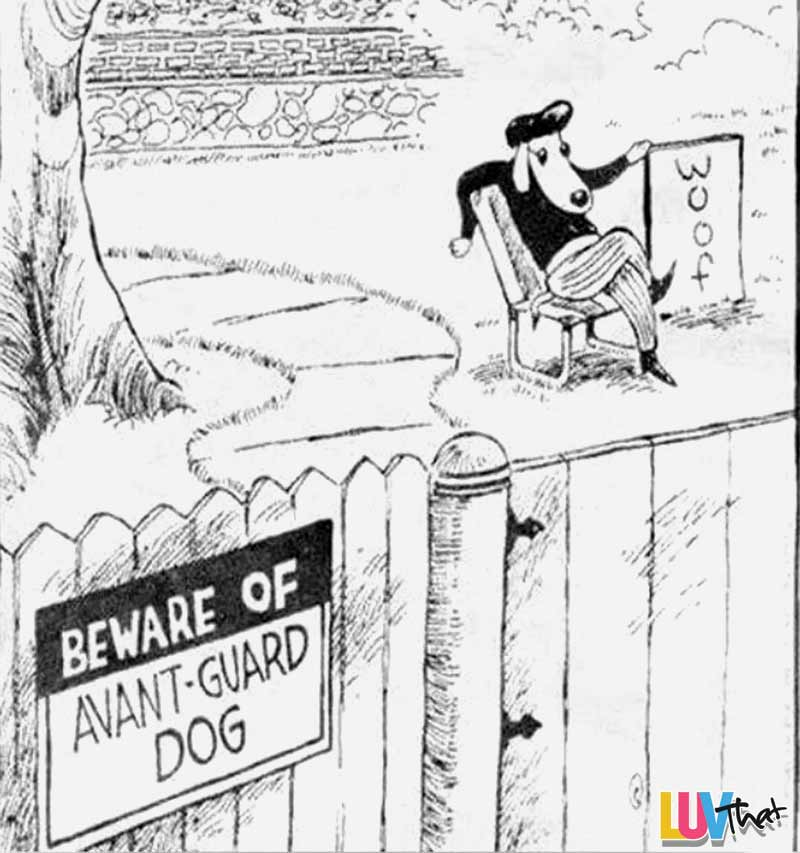
\includegraphics[scale=0.28]{./BewareTheAvantGuardDog.jpg}
  \end{figure}
\end{frame}

\begin{frame}
  \frametitle{iClicker Question}
Choose from the following options. This item will be graded.
\begin{block}{iClicker Question}
Which philosopher's work on writing and figurative speech does Derrida
use as his starting point for his own reflections?
\end{block}
\begin{description}
\item[A\hspace{.2in}$\blacktriangleright$] Jean-Jacques Rousseau
\item[B\hspace{.2in}$\blacktriangleright$] Jean-Paul Sartre
\item[C\hspace{.2in}$\blacktriangleright$] Michel Foucault
\item[D\hspace{.2in}$\blacktriangleright$] Voltaire
\end{description}
\end{frame}

\begin{frame}
  \frametitle{iClicker Question}
Choose from the following options. This item will be graded.
\begin{block}{iClicker Question}
Which analogy (or origin) does Derrida use to show how the practice of
writing won out over the practice of reading?
\end{block}
\begin{description}
\item[A\hspace{.2in}$\blacktriangleright$] space travel (satellites)
\item[B\hspace{.2in}$\blacktriangleright$] alchemy and chemistry (production of ink)
\item[C\hspace{.2in}$\blacktriangleright$] musical notation (staves)
\item[D\hspace{.2in}$\blacktriangleright$] agriculture (ploughs and furrows)
\end{description}
\end{frame}

\begin{frame}
  \frametitle{iClicker Question}
Choose from the following options. This item will be graded.
\begin{block}{iClicker Question}
Where, according to Barthes, does the text assume a measure of unity
and focus?
\end{block}
\begin{description}
\item[A\hspace{.2in}$\blacktriangleright$] in the reader
\item[B\hspace{.2in}$\blacktriangleright$] in the author
\item[C\hspace{.2in}$\blacktriangleright$] in the narrator
\item[D\hspace{.2in}$\blacktriangleright$] in the writer
\end{description}
\end{frame}

\begin{frame}
  \frametitle{iClicker Question}
Choose from the following options. This item will be graded.
\begin{block}{iClicker Question}
Which of these triplets does not reflect the three stages of society in Derrida/Rousseau?
\end{block}
\begin{description}
\item[A\hspace{.2in}$\blacktriangleright$] savage/barbaric/civil
\item[B\hspace{.2in}$\blacktriangleright$] pictography/hieroglyphs/alphabet
\item[C\hspace{.2in}$\blacktriangleright$] fetishism/polytheism/monotheism
\item[D\hspace{.2in}$\blacktriangleright$] hunter/shepherd/ploughman
\end{description}
\end{frame}

\begin{frame}
  \frametitle{Writing}
  Note how Derrida uses the hermeneutic method to explain his ideas:
  always in relation to already existing texts (Rousseau, Warburton,
  Condillac, Malebranche).
  \begin{quote}
    But the importance of these two chapters, the obstinate effort to
    consolidate a theory, the laborious ruse to disqualify the
    interest given to writing, are signs that one may not
    neglect. Such is the situation of writing within the history of
    metaphysics: a debased, lateralized, repressed, displaced theme, yet
    exercising a permanent and obsessive pressure from the place where
    it remains held in check. A feared writing must be crossed out
    because it erases the presence of the proper within speech. (292)
  \end{quote}
\end{frame}

\begin{frame}
  \frametitle{Contrasts}
  \begin{tabular}{rcl}
      feelings & vs & ideas \\
      South & vs & North \\
      vowels & vs & consonants \\
      figurative & vs & literal \\
      passion & vs & need \\
      savage metaphor & vs & idea metaphor \\
      savagery & vs & civility (transference, interval) \\
      state of nature & vs & state of society (happy pause, 304) \\
      pictography & vs & algebra (two simplicities, 310) \\
  \end{tabular}
\end{frame}

\begin{frame}
  \frametitle{Contrasts}
  \begin{quote}
    The progress of writing is thus a natural progress. And it is a
    progress of reason {\ldots} why is that dangerous progress
    natural? No doubt because it is necessary {\ldots} it is need and
    not passion that substitutes light for heat, clarity for desire,
    precision for strength, ideas for sentiment, reason for heart,
    articulation for accent. (295)
  \end{quote}  
\end{frame}

\begin{frame}
  \frametitle{Concepts}
  \begin{description}
  \item[savage metaphor] the metaphor which is not preceded by
    anything (giants): no literal or proper meaning precedes it, no
    rhetor watches over it (301)
    \item[rhetor] the rhetor accedes to objective truth, denounces
      error, deals with the passions, but all by virtue of having lost
      the living truth of the origin {\ldots} the enlightened spirit
      stabilizes the literal meaning, and does it by a process of
      knowledge and in terms of truth (302) (truth is only one epoch,
      implying the presence of the signified, see 312)
    \item[noun] the work which produces the common noun supposes, like
      all work, the chilling and displacement of passion (303)
    \item[transference] the interval between the thing itself and its
      reproduction (307)
  \end{description}
\end{frame}

\begin{frame}
  \frametitle{Festival Around the Water Hole}
  \begin{quote}
    A language without discourse, a speech without sentence, without
    syntax, without parts, without grammar, a language of pure
    effusion, beyond the cry, but short of the hinge that articulates
    and at the same time disarticulates the immediate unity of meaning
    (304)
  \end{quote}
  Is Rousseau mistaking ontogenesis with phylogenesis here (absorption
  into the present moment, 336)? ``{\ldots} a world alien to the
  trace: pure presence of the pure present'' (316).
      \begin{quote}
        These innocent spectacles will take place outdoors and they
        will have nothing ``effeminate'' or ``mercenary'' about them.
        The sign, money, ruse, passivity, and servility will be
        excluded from them. No one will use anyone, no one will be an
        object for anyone. (333, the London gay club in Foucault)
      \end{quote}
\end{frame}

\begin{frame}
  \frametitle{The Onto-Theological Idea of Experience}
      The epoch of logocentrism is a moment of the global effacement
      of the signifier: one then believes one is protecting and
      exalting speech, one is only fascinated by a figure of the
      \emph{techn{\`e}} (311).
  \begin{quote}
    The very concept of experience remains dependent on the
    idea of original sin. There is one law there: the notion of
    experience, even when one would like to use it to destroy
    metaphysics or speculation, continues to be, in one or another
    point of its functioning, fundamentally inscribed with in onto-theology:
    at least by the value of \emph{presence}, whose implication
    it can never reduce by itself. Experience is always the
    relationship with a plenitude, whether it be sensory simplicity
    or the infinite presence of God. (308)
  \end{quote}
\end{frame}

\begin{frame}
  \frametitle{Supplanting}
  The word ``supplant'' well defines the act of writing (305). The
  ``supplement gives itself as supplement of supplement, sign of
  sign.'' 
  \begin{quote}
    The supplement is always the supplement of a supplement. One
    wishes to go back from the supplement to the source: one must
    recognize that there is a supplement at the source. (330)
  \end{quote}
\end{frame}

\begin{frame}
  \frametitle{The Role of Philosophy}
  \begin{quote}
    A writing within which philosophy is inscribed as a place within
    a text which it does not command. Philosophy is, within writing,
    nothing but this movement of writing as effacement of the
    signifier and the desire of presence restored, of being, signified
    in its brilliance and its glory. (311f)
  \end{quote}
  Philosophy is the ``invention of prose'' (312). 
\end{frame}

\begin{frame}
  \frametitle{Representation}
  Representation in politics and in writing: the culture of the
  alphabet and the appearance of civilized man (326). In capitalism,
  there is an arbitrary sign which is superior to all non-arbitrary
  representors: money. Writing also is superior to the voice in
  representing; at the same time, it is a ``machine of death'' (327).
  Overwhelming success 
  \begin{block}{Jean-Jacques Rousseau: Fragment on Pronuncation}
    results in our having nothing to say to others except the least
    interesting things in the world and things that they care least to
    understand: sermons, academic discourses. (328)
  \end{block}
\end{frame}

\begin{frame}
  \frametitle{The Essence of the Supplement}
  Derrida says repeatedly that the supplement is necessary. ``The
  progress of writing is necessary'' (295). 
  \begin{quote}
    Not to attribute any necessity to the historical appearance of
    writing is at once to ignore the appeal of supplanting and to
    think evil as a surprising, exterior, irrational, accidental
    addition and therefore effaceable. (321)
  \end{quote}
  On page 341, however, he also claims that ``the strange essence of
  the supplement is not to have essentiality: it may always not have
  taken place.'' What gives? ``The supplement is neither a presence
  nor an absence. No ontology can think its operation'' (342).
\end{frame}

\begin{frame}
  \frametitle{Death of the Author}
See marked-up pdf file.  
\end{frame}

\end{document}
